\documentclass[../notes.tex]{subfiles}
\begin{document}
\section{Day 4}
    \subsubsection{Definition of Fundamental Group}
    \begin{itemize}
        \item \underline{Recall:} If,
            \begin{align*}
                f&=\text{path in $X$ from x to y}\\
                g&=\text{path in $X$ from y to z}\\
            \end{align*}
            Then,
            \begin{align*}
                [f]*[g]:=[\text{concatenation $f*g$ of $f$ and $g$}]\\
            \end{align*}
        \item{Properties of $*$:}
            \begin{enumerate}
                \item $*$ is associative, or
                    \begin{align*}
                        [f]*([g]*[h])=([f]*[g])*[h]\\
                    \end{align*}
                    The idea here is that we can adjust the time taken to travel on the path.
                    These two paths are path-homotopic: interpolate between $f*(g*h)$ and
                    $(f*g)*h$ by making f take less and less time and h take more and more time.\\
            \begin{minipage}[c]{\linewidth}
                \begin{center}
                    \begin{tikzpicture}
                        \begin{axis}[
                            width=\linewidth, height=8cm,
                            ticks=none,
                            ymin=-1,ymax=1
                            ]
                            \draw (20,170) node {$(\textcolor{blue}{f}*\textcolor{green}{g})*\textcolor{red}{h}$};
                            \addplot [samples=200, domain=0:1,color=blue] {-.25*cos(deg(6.28*x))}
                            node [pos=.5,below,yshift=-5mm] {$f$};
                            \draw [decorate,decoration={brace,amplitude=20pt, mirror},color=blue] (0,65) -- (100,65)
                            node [pos=.5, below, yshift=-8mm, color=blue] {$0\leq s \leq\frac{1}{4}$};

                            \addplot [samples=200, domain=1:2,color=green] {-.25*cos(deg(6.28*x))}
                            node [pos=.5,below,yshift=-5mm] {$g$};
                            \draw [decorate,decoration={brace,amplitude=20pt, mirror},color=green] (100,65) -- (200,65)
                            node [pos=.5, below, yshift=-8mm, color=green] {$\frac{1}{4}\leq s \leq\frac{1}{2}$};

                            \addplot [samples=200, domain=2:3,color=red] {-.25*cos(deg(6.28*x))}
                            node [pos=.5,below,yshift=-5mm] {$h$};
                            \draw [decorate,decoration={brace,amplitude=20pt, mirror},color=red] (200,65) -- (300,65)
                            node [pos=.5, below, yshift=-8mm, color=red] {$\frac{1}{2}\leq s \leq 1$};
                        \end{axis}
                    \end{tikzpicture}
                \end{center}
            \end{minipage}\\
            \begin{minipage}[c]{\linewidth}
                \begin{center}
                    \begin{tikzpicture}
                        \begin{axis}[
                            width=\linewidth, height=8cm,
                            ticks=none,
                            ymin=-1,ymax=1
                            ]
                            \draw (20,170) node {$\textcolor{blue}{f}*(\textcolor{green}{g}*\textcolor{red}{h})$};
                            \addplot [samples=200, domain=0:1,color=blue] {-.25*cos(deg(6.28*x))}
                            node [pos=.5,below,yshift=-5mm] {$f$};
                            \draw [decorate,decoration={brace,amplitude=20pt, mirror},color=blue] (0,65) -- (100,65)
                            node [pos=.5, below, yshift=-8mm, color=blue] {$0\leq s \leq\frac{1}{2}$};

                            \addplot [samples=200, domain=1:2,color=green] {-.25*cos(deg(6.28*x))}
                            node [pos=.5,below,yshift=-5mm] {$g$};
                            \draw [decorate,decoration={brace,amplitude=20pt, mirror},color=green] (100,65) -- (200,65)
                            node [pos=.5, below, yshift=-8mm, color=green] {$\frac{1}{2}\leq s \leq\frac{3}{4}$};

                            \addplot [samples=200, domain=2:3,color=red] {-.25*cos(deg(6.28*x))}
                            node [pos=.5,below,yshift=-5mm] {$h$};
                            \draw [decorate,decoration={brace,amplitude=20pt, mirror},color=red] (200,65) -- (300,65)
                            node [pos=.5, below, yshift=-8mm, color=red] {$\frac{3}{4}\leq s \leq 1$};
                        \end{axis}
                    \end{tikzpicture}
                \end{center}
            \end{minipage}
                \item $*$ has left/right identities.\\
                    Let
                    \begin{align*}
                        e_x&: I\rightarrow X\\
                        e_x(s)&=x,\ \forall\ s\in I, \text{``constant path at $x$''}\\
                    \end{align*}
                    Then, for all paths $f$ from $x$ to $y$, $[f]*[e_y]=[f]$, and
                    $[e_x]*[f]=[f]$. The premise here is that $e_x$ or $e_y$ spend "half
                    the time" sitting at either $x$ or $y$.\\
                    \begin{minipage}[c]{\linewidth}
                        \begin{center}
                            \begin{tikzpicture}
                                \begin{axis}

                                \end{axis}
                            \end{tikzpicture}
                            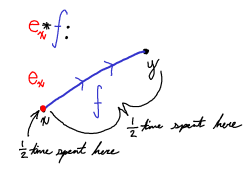
\includegraphics[]{images/path_identity.png}
                        \end{center}
                    \end{minipage}
                    These are path-homotopic: interpolate between $f*e_y$ and $f$ by making
                    $f$ take longer and longer.
                \item $*$ has inverses.\\
                    Let $f$ be a path from $x$ to $y$, and let $\overline{f}$ be the ``reverse'' path,
                    \begin{align*}
                        \overline{f}(s)=f(1-s)\\
                    \end{align*}
                    Then,
                    \begin{align*}
                        [f]*[\overline{f}]&=[e_x]\\
                        [\overline{f}]*[f]&=[e_y]\\
                    \end{align*}\\
                    \begin{minipage}[c]{\linewidth}
                        \begin{center}
                            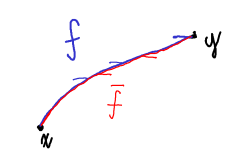
\includegraphics[]{images/path_inverse.png}
                        \end{center}
                    \end{minipage}
                    \underline{Idea:} 
                    The verbal gist of this is that the path takes half the time to travel to its destination, and
                    is concatenated with a path that spends half the time to travel to the origin of the original
                    function.\\
            \end{enumerate}
        \item
            These are path-homotopic: interpolate between $f*\overline{f}$ and $e_x$ by doing less and less
            of $f$ before turning around.
        \item Let,
            \begin{align*}
                X&=\text{topological space}\\
                x&\in X\\
            \end{align*}
            \begin{definition} A \underline{loop} in $X$ based at $x\in X$ is a path,
            \begin{align*}
                f:I&\rightarrow X\\
                \text{such that}
                &f(0)=f(1)\\
            \end{align*}
            \end{definition}
            \begin{minipage}[c]{\linewidth}
                \begin{center}
                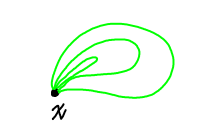
\includegraphics[]{images/loops.png}
                \end{center}
            \end{minipage}
        \item \underline{Observation:} If $f$ and $g$ are any two loops in $X$ based at $x$,
            then $f*g$ is a loop.
    \end{itemize}
            \begin{definition}
                The \underline{fundamental group} of the $X$ with basepoint $x$ is:
                \begin{align*}
                    \pi(X,x)=\{\text{path-homotopy classes of loops in $X$ based at $x$}\}\\
                \end{align*}
                This is a group with the operation $*$\\
            \end{definition}
    \begin{itemize}
        \item $e_x$ and $e_y$ are loops.
        \item $f*\overline{f}$ and $\overline{f}*f$ are also loops.
        \item \underline{Note:} The fact that $\pi_1(X,x)$ satisfies the axioms of a group, and follows from the
            properties of $*$ we just checked.\\
            (E.g. the identity element is $[e_x]$)\\
        \item \underline{Question:} What is $\pi_1(\R^2, (0,0))$?\\
            Do you have a guess for $\pi_{1}(S', (1,0))$?\\
            Answer 1: $\pi_1(\R^2, (0,0))\cong \{1\}$\\
            To prove this, it's enough to show that $\pi_1(\R^2, (0,0))$ has just one element,\\
            i.e., any loop in $\R^2$ based at $(0,0)$, is path-homotopic to any other. This is true
            via the straight line homotopy.
            Answer 2: $\pi_1(S', (1,0))\cong \Z$.\\
    \end{itemize}
\end{document}
